%preamble
\documentclass[6pt]{article}
\usepackage[absolute,[DEBUG]]{textpos}
\usepackage{setspace}
\usepackage{graphicx}
\usepackage{colortbl}
\usepackage{times}
\usepackage{array}
\usepackage[none]{hyphenat}
\setlength{\TPHorizModule}{1cm}
\setlength{\TPVertModule}{\TPHorizModule}
\textblockorigin{0.1cm}{0.1cm} % start everything near the top-left corner
%End preamble
\begin{document}
\fontfamily{phv}
\selectfont

\begin{textblock}{13.75}(0,2.1)
Origin Time: [ORIGTIME] UTC ([LOCALTIME] local) 
\end{textblock}

\begin{textblock}{5.5}(7.2,-0.2)
\includegraphics[scale=0.18]{[VERSIONFOLDER]/alertsponge.pdf}
\end{textblock}
\begin{textblock}{3.2}(0,0.3)

\includegraphics[scale=0.17]{[HOMEDIR]/losspager/logos/USGSid.pdf}
\end{textblock}
\begin{textblock}{1.1}(14.9,0.3)

\includegraphics[scale=0.30]{[HOMEDIR]/losspager/logos/GSN.pdf}
\end{textblock}
\begin{textblock}{1.8}(14.9,1.4)

\includegraphics[scale=0.15]{[HOMEDIR]/losspager/logos/ANSS_cropped_bw.pdf}
\end{textblock}
\begin{textblock}{3.75}(16.2,0.3)

\includegraphics[scale=0.59]{[HOMEDIR]/losspager/logos/USAID.pdf}
\end{textblock}
\begin{textblock}{13.75}(0,12.65)
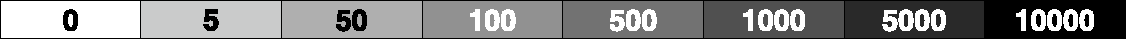
\includegraphics[scale=0.691]{[HOMEDIR]/losspager/logos/population_scale.pdf}
\end{textblock}
\begin{textblock}{13.75}(0,13.1)
\includegraphics[scale=0.96,width=[EXPWIDTH]cm,height=[EXPHEIGHT]cm]{[VERSIONFOLDER]/exposure.pdf}
\end{textblock}

\begin{textblock}{13.75}(0,1.6)
\fontsize{15}{18}\textbf{[MAGLOC]}
\end{textblock}



\begin{textblock}{13.75}(0,2.5)
Location: [LAT]$\,^{\circ}$[HEMILAT] [LON]$\,^{\circ}$[HEMILON] Depth: [DEPTH] km
\end{textblock}

\begin{textblock}{18}(0,2.9)
{\color{red}\textbf{[TSUNAMI]}}
\end{textblock}

\begin{textblock}{8}(18.2,1.6)
\fontsize{15}{18}\textbf{PAGER}
\end{textblock}

\begin{textblock}{8}([VERSIONX],2.2)
\fontsize{15}{18}\textbf{[VERSION]}
\end{textblock}

\begin{textblock}{12}([ELAPSEDX],2.9)
[ELAPSED]
\end{textblock}

\begin{textblock}{8}(0.1,3.6)
\fontsize{14}{16.8}\textbf{Estimated Fatalities}
\end{textblock}

\begin{textblock}{5.5}(7.5,3.2)
\begin{spacing}{0.8}
\begin{flushleft}
{\small [IMPACT1]}
\end{flushleft}
\end{spacing}
\end{textblock}

\begin{textblock}{6.1}(7.5,5.6)
\begin{spacing}{0.8}
\begin{flushleft}
{\small [IMPACT2]}
\end{flushleft}
\end{spacing}
\end{textblock}

\begin{textblock}{13.75}(0.1,4.0)
\includegraphics[scale=0.18]{[VERSIONFOLDER]/alertfatal.pdf}
\end{textblock}

\begin{textblock}{13.75}(13.1,4.0)
\includegraphics[scale=0.18]{[VERSIONFOLDER]/alertecon.pdf}
\end{textblock}

\begin{textblock}{8}(13.1,3.6)
\fontsize{14}{16.8}\textbf{Estimated Economic Losses}
\end{textblock}

\linethickness{2pt}
\begin{textblock}{21}(0,3.3)
\line(1,0){569.4}
\end{textblock}

\begin{textblock}{21}(-0.01875,7.5)
\line(1,0){571.15}
\end{textblock}

\begin{textblock}{1}(0.532,3.3)
\line(0,1){120}
\end{textblock}

\begin{textblock}{1}(20.55,3.3)
\line(0,1){120}
\end{textblock}

\begin{textblock}{10}(0,11.75)
{\footnotesize *Estimated exposure only includes population within the map area}
\end{textblock}

\begin{textblock}{7.5}(0,12.1)
\fontsize{14}{16.8}\textbf{Population Exposure}
\end{textblock}

\begin{textblock}{7.5}(8.2,12.3)
{\footnotesize population per ~1 sq. km from Landscan}
\end{textblock}
\begin{textblock}{7.5}(13.37,12.28)
\fontsize{9}{16.8}\textbf{Structures:}
\end{textblock}

\begin{textblock}{6.5}(13.9,12.30)
\begin{spacing}{0.85}
\begin{flushleft}
{\small [STRUCTCOMMENT]}
\end{flushleft}
\end{spacing}
\end{textblock}

\begin{textblock}{17}(0,7.7)
\fontsize{14}{16.8}\textbf{Estimated Population Exposed to Earthquake Shaking}
\end{textblock}

\begin{textblock}{20}(0,8.1)
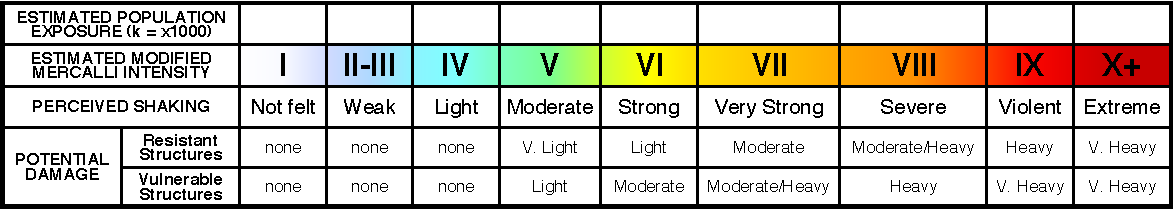
\includegraphics[width=20.05cm]{[HOMEDIR]/losspager/logos/exptable.pdf}
\end{textblock}

\begin{textblock}{1.5}([MMI1X],8.35)
  [MMI1]
\end{textblock}

\begin{textblock}{1.5}([MMI2-3X],8.35)
  [MMI2-3]
\end{textblock}

\begin{textblock}{1.5}([MMI4X],8.35)
  [MMI4]
\end{textblock}

\begin{textblock}{1.5}([MMI5X],8.35)
  [MMI5]
\end{textblock}

\begin{textblock}{1.5}([MMI6X],8.35)
  [MMI6]
\end{textblock}

\begin{textblock}{1.5}([MMI7X],8.35)
  [MMI7]
\end{textblock}

\begin{textblock}{1.5}([MMI8X],8.35)
  [MMI8]
\end{textblock}

\begin{textblock}{1.5}([MMI9X],8.35)
  [MMI9]
\end{textblock}

\begin{textblock}{1.5}([MMI10X],8.35)
  [MMI10]
\end{textblock}

\begin{textblock}{7.5}(13.4,15.6)
\textbf{Historical Earthquakes (with MMI levels):}
\end{textblock}

[HISTORICAL_BLOCK]

\begin{textblock}{7.5}(13.4,20.2)
\fontsize{14}{16.8}\textbf{Selected City Exposure}
\end{textblock}

\begin{textblock}{7.5}(13.4,20.7)
{\footnotesize from GeoNames.org}
\end{textblock}


\begin{textblock}{7.8}(13.4,21.05)
[CITYTABLE]
\end{textblock}

\begin{textblock}{13.0}(0.0,26.35)
{\footnotesize PAGER content is automatically generated, and only considers losses due
to structural damage.}
\end{textblock}

\begin{textblock}{12.0}(0.0,26.65)
{\footnotesize Limitations of input data, shaking estimates, and loss models 
may add uncertainty.}
\end{textblock}

\begin{textblock}{7.5}(13.4,[CITYFOOTERHEIGHT])
{\footnotesize bold cities appear on map}
\end{textblock}

\begin{textblock}{7.5}(18.80,[CITYFOOTERHEIGHT])
{\footnotesize (k = x1000)}
\end{textblock}

\begin{textblock}{7.5}(0.0,27.1)
{\footnotesize \textbf{http://earthquake.usgs.gov/pager}}
\end{textblock}

\begin{textblock}{7.5}([EVENTIDX],27.1)
\textbf{[EVENTID]}
\end{textblock}

\end{document}